\chapter{Future Research: Non-Parametric Sequential Decision Making in Non-Euclidian Spaces}
\label{chapter:future-research}


\section{Introduction}
To date, my research has focussed on using Gaussian processes (GPs) as building blocks for deep models, similar to neural network layers. In this vein, I have worked on (1) deep convolutional Gaussian processes that mimic the convolutional and layered architectures encountered in many contempory deep learning models \citep{Dutordoir2020convolutional}, (2) conditional density estimation models which are similar to Variational Auto Encoders \citep{dutordoir2018cde,Salimbeni2019}, and (3) more recently, deep Gaussian processes that have basis functions that are similar to neural network activation functions \citep{dutordoir2021deep} (discussed at length in \cref{chapter:dnn-as-point-estimate-for-dgps}). I have packaged these advances in a software toolbox, called GPflux \citep{dutordoir2021gpflux}, that provides these GP layers through a neueral network like interface. The main advantage of this approach is that straightforward application of Bayesian principles leads to sensible results, which is not the case for normal neural networks [TODO CITE Wenzel]. The current state of research into using Gaussian processes as layers is that classification performance starting to be on-par with deep learning on simple datasets \citep{dutordoir2018cde}, but with good uncertainty quantification and automatic selection of hyperparameters working `out of the box'.

The primary focus of my previous research can be considered as `curve-fitting', i.e. finding the best function approximator when given examples of inputs and corresonponding outputs. In this setting we can consider two regimes: (1) the function is very complex but there is an abundance of (high-quality) data to learn the mapping, and (2) the function is of a simpler nature but the underlying data is limited, noisy and/or very expensive to acquire. As evidenced by many recent advances in domains where there is an abundance of data, such as natural language, generative modelling and vision, the first regime is a setting where deep learning models thrives. Indeed, the natural inductive bias of deep neural networks (DNNs) in combination with the low computational cost of training them on massive datasets has proven to be very effective. Arguably, performing (approximate) Bayesian inference in this regime will contribute little to the end result. The second regime, however, in which data is limited and noisy, requires a completely different modelling paradigm. In this setting, a model needs to be uncertain about which information they can deduct from the training data, be able to update the current belief in lights of new data ---even a single datapoint--- and be able to generalise well from limited data. In this setting one typically want to use these models to drive decisions. BAYESIAN FRAMEWORK TODO.  I believe that this is a setting that has been understudied and undervalued in the recent deep learning `hype', yet it is of high importance in many scientific and commercial applications. In what comes next in my PhD I would like to focus on this regime.

% Through this line of work, I believe that we have showed that (deep) Gaussian processes are an interesting non-parametric alternative to Bayesian neural networks (BNNs). Our work differs from the conventional BNN literature in that we attempt to scale well-understood fully-Bayesian models (i.e. GPs) to big data settings, rather than the converse: starting from complex parametric models and trying to approximate Bayesian inference in them. The former strategy allows to gradually build up complexity into the models while maintaining their favourable properties, such as a marginal likelihood objective and good uncertainty quantifications.

% In what comes next, I want to separate the different regimes in which neural networks and Gaussian processes operate and thrive. For example, NNs can handle---and in practice require---very large datasets, whereas Gaussian process models are more comfortable in the small data regime. Neural networks, in the presence of large datasets, are extremely good at learning complex latent representations, as evidenced by the latest models in natural language processing and computer vision. Non-parametric Gaussian processes, on the contrary, work best on limited and noisy datasets. Datasets where each datapoint can be very expensive in terms of cost or time to obtain. I believe that this is a setting---in the era of deep learning---that has been under studied and valued, yet of high importance for many scientific or commercial applications.

% Many real-world problems can be described as inferring properties of an expensive black-box function $f: \mathcal{X} \rightarrow \mathcal{Y}$, subject to a computational budget of $T$ function evaluations. Typical examples are (global) optimisation, finding a level set (i.e. the set of points in $X \subset \mathcal{X}$ for which $f(x) > C,\forall x \in X$), or finding the shortest path between two nodes in a graph. In the graph example, the black-box function $f$ would return the cost of traversing an edge and query the cost of an edge would be very expensive. Naively applying Dijkstra would require the evaluation of $f$ at every edge and thus potentially grossly exceeding the given budget of $T$ evaluations.

\section{Background}

Bayesian models should be developed with their use-case in mind. A general use case is that of sequential decision making, which encapsulates a wide range of real-worlds problem settings. In the most general terms, a MDP consists of the following components 
Sequential decision making
\begin{enumerate}
    \item State space
    \item Action space
    \item Reward probability
    \item Transition probability
\end{enumerate}

\subsection{Examples}
\paragraph{Bayesian optimisation}
\paragraph{Contextual multi-armed bandits}


\section{Gaussian processes as surrogate model in non-Euclidian manifolds}

% \begin{enumerate}
%     \item Low dimensions
%     \item Prior knowledge
%     \item Limited, noisy and very expensive data
%     \item Non-Euclidian spaces: graphs, meshes, and closed manifolds (e.g. circle).
% \end{enumerate}

Stationary kernels are ubiquitous in Gaussian processes when the input space is Euclidean. 


manifolds 
Descrete cases: undirected graph and meshes

Define Matern kernels:
\begin{equation}
    k(x, x) = \sum_i S(\sqrt{\lambda_i}) \phi_i(x) \phi_i(x')
\end{equation}

We want to place a \emph{surrogate model} between the expensive function $f$ and the algorithm. We model $\tilde{f}$ by a Gaussian process
\begin{equation}
    \tilde{f} \sim \GP
\end{equation}

\subsection{Research Questions}


\section{Applications}

\begin{enumerate}
    \item Bayesian search: airplane crash -> gravitational waves
\end{enumerate}


% Basically settings where DNNs are never going to be competitive with GPs - low-dim, very data-efficient, high-cost - not even if someone figures out how to do DNN uncertainty right, due to GP regret guarantees (under reasonable assumptions) matching the best possible regret achievable by any model/decision system.

\paragraph{Related areas}
\begin{enumerate}
    \item Probabilistic numerics [Tubingen Manifesto, Osborne and Henning]. They are less interested in closing the loop and making decisions atop of the models. They usually plot the error bars on the estimator as their final result.
    \item Bayesian optimisation methods. Special case.
\end{enumerate}

% \paragraph{Real-world problems}
% \begin{itemize}
%     \item[Graphs] Social networks. Search for cliques or shortest paths.
%     \item[Meshes] Aerospace and civil engineering problems. ``General'' sensor placement.
%     \item[Manifold] Sphere. Interesting problem in astrophysics: when a gravitational wave detection is made there's usually a very large uncertainty of its origin so optical telescopes have to sweep the sky looking for the source.
% \end{itemize}

% \paragraph{Objectives}
% \begin{enumerate}
%     \item Theory and analysis
%     \item Show the excellence of Gaussian processes in this regime
%     \item Benchmarks for future methods
% \end{enumerate}

% \paragraph{Practical}
% \begin{enumerate}
%     \item Collaborators
%     \begin{enumerate}
%     \item Alex Terenin (Imperial College London), currently with Marc Deisenroth but starting post-doc at Cambridge.
%     \item Willie Neiswanger (Stanford University), with prof. Stefano Ermon.
%     \end{enumerate}
%     \item We need to find the right problems to solve, which can take time.
% \end{enumerate}

% \begin{enumerate}
%     \item Black Box Functions $f: \mathcal{X} \rightarrow \mathcal{Y}$
%     \item We want to estimate a computable property $\mathcal{O}_\mathcal{A}(f)$
%     \item $\mathcal{A}$ is an algorithm $\mathcal{O}_\mathcal{A}(f) = \mathcal{A}(f)$
%     \item Evaluating $f$ is \emph{very} expensive (we can only evaluate it a limited amount of times)
% \end{enumerate}

% \paragraph{Examples}
% \begin{enumerate}
%     \item Optimisation: $\mathcal{A}(f) = \argmax_{x\in\mathcal{X}} f(x)$, which implies $\mathcal{O}_\mathcal{A}(f) = x^*$.
%     \item Sensor Placement (Active Learning): $\mathcal{O}_\mathcal{A}(f) = \argmax_{X \subset \mathcal{X}, |X| = T} \textrm{MI}(f, f(X))$.
%     \item Level sets: $\mathcal{O}_\mathcal{A}(f) = \{X \subset \mathcal{X}: f(x) > C, \forall x \in X\}$.
%     \item Shortest path: $\mathcal{O}_\mathcal{A}(f) = $ shortest path between two nodes in a graph.
% \end{enumerate}



% \section{On-going Projects}

% \begin{enumerate}
%     \item ``Pay Attention to Deep Gaussian Processes''\\
%     Transformer Layer Gaussian Processes using an explicit feature representation of the attention operation. The inducing points would play the role of keys in the attention layer.
%     \begin{equation*}
%         \exp(\vx^\top \vy) = \Phi^\top(\vx) \Phi(\vy)
%     \end{equation*}
%     % \begin{equation*}
%     %     \exp(\vx^\top \vy) = \Phi^\top(\vx) \Phi(\vy)
%     % \end{equation*}
%     \item Green's Inducing Functions for GPs in Balls
%     \begin{enumerate}
%         \item Indcing points: adaptivity
%         \item Variational Fourier Features: boundary conditions, doesn't scale with dimensionality
%         \item Variational Orthogonal Features: 
%         \item Spherical Harmonics: restricted in kernel, diagonal Kuu
%     \end{enumerate}
%     \item VISH-PI: Probabilistic Integration with Variational Inducing Spherical Harmonics, with Michael Osborne and Saad Hamid (student)
% \end{enumerate}


% % \begin{figure}[htb]
% %     \centering % <-- added
% % \begin{subfigure}{0.25\textwidth}
% %   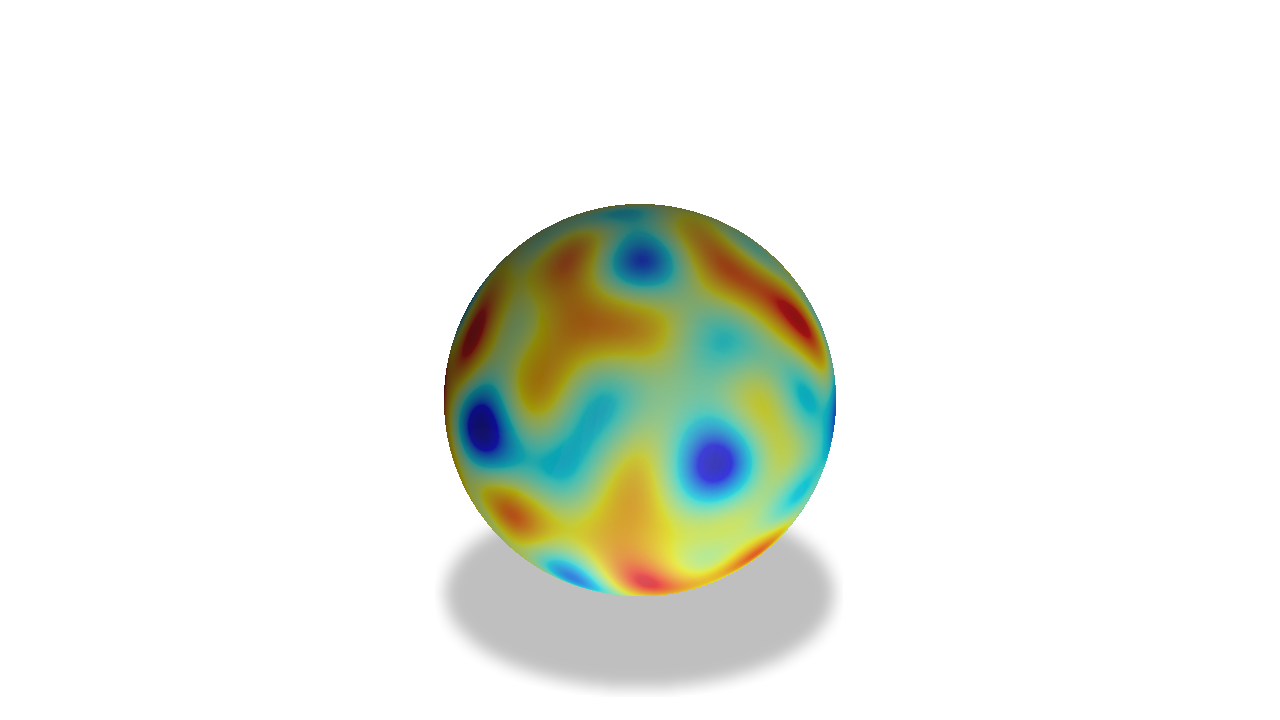
\includegraphics[width=\linewidth]{Chapter5/figures/sphere.png}
% % %   \caption{Manifolds}
% %   \label{fig:1}
% % \end{subfigure}\hfil % <-- added
% % \begin{subfigure}{0.25\textwidth}
% %   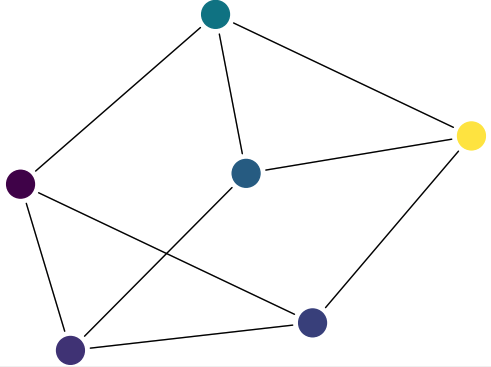
\includegraphics[width=\linewidth]{Chapter5/figures/graph.png}
% % %   \caption{Graphs}
% %   \label{fig:2}
% % \end{subfigure}\hfil % <-- added
% % \begin{subfigure}{0.25\textwidth}
% %   \includegraphics[width=\linewidth]{Chapter5/figures/BunnyWire.png}
% % %   \caption{Meshes}
% %   \label{fig:3}
% % \end{subfigure}

% % \medskip
% % \begin{subfigure}{0.25\textwidth}
% %   \includegraphics[width=\linewidth]{Chapter5/figures/cosmos.png}
% % %   \caption{Cosmos}
% %   \label{fig:4}
% % \end{subfigure}\hfil % <-- added
% % \begin{subfigure}{0.25\textwidth}
% %   \includegraphics[width=\linewidth]{Chapter5/figures/social_network.png}
% % %   \caption{image5}
% %   \label{fig:5}
% % \end{subfigure}\hfil % <-- added
% % \begin{subfigure}{0.25\textwidth}
% %   \includegraphics[width=\linewidth]{Chapter5/figures/mesh_engine.png}
% % %   \caption{image6}
% %   \label{fig:6}
% % \end{subfigure}
% % \caption{Domains (top) and applications (bottom)}
% % \label{fig:images}
% % \end{figure}
